Comparing $y^2=4x$ to standard equation,
\begin{align}
ax^2+2bxy+cy^2+2dx+2ey+f = 0
\end{align}
$\therefore$ a = b = e = 0, d =-2, c = 1, f = 0.
\begin{align}
\therefore \vec{V} = \myvec{a&b\\b&c} = \myvec{0&0\\0&1}
\end{align} 
\begin{align}
\therefore\vec{u} = \myvec{d\\e} = \myvec{-2\\0}\label{eq:solutions/1/20/u}
\end{align}
\begin{align}
 \mbox{ Now,} \mydet{V} = \mydet{0&0\\0&1} = 0
\end{align}
$\implies$ That the curve is a parabola.
\begin{align}
    \mbox{Since} \ \vec{V}\vec{p_1}=0\\
    \therefore \vec{p_1}=\myvec{1\\0}
\end{align}
Since the slope of the line is 1
The direction vector $\vec{m}$ is as follows:
\begin{align}
\vec{m} = \myvec{1\\1}
\end{align}
\begin{align}
    \mbox{Since} \ \vec{m}^T\vec{n}=0 \\
    \therefore \vec{n} = \myvec{1\\-1}\label{eq:solutions/1/20/n}
\end{align} 
Now, the equation for the point of contact for the parabola is given as,
\begin{align}
\myvec{\vec{u}^T+\kappa\vec{n}^T\\\vec{V}}\vec{q} = \myvec{-f\\\kappa\vec{n}-\vec{u}}\label{eq:solutions/1/20/contact}\\
\mbox{where, } \kappa = \frac{\vec{p_1}^T\vec{u}}{\vec{p_1}^T\vec{n}} = -2 \label{eq:solutions/1/20/k}
\end{align}
By substituting the values ,we get:
\begin{align}
\myvec{-4&2\\0&0\\0&1}\vec{q} = \myvec{0\\0\\2}
\label{eq:solutions/1/20/solve_q}
\end{align}
Solving for $\vec{q}$ by removing the zero row and representing \eqref{eq:solutions/1/20/solve_q} as augmented matrix and then converting the matrix to echelon form,
\begin{align}
\implies \myvec{-4&2&0\\0&1&2} \xleftrightarrow[]{R_1\leftarrow\brak{\frac{-R_1}{4}}} \myvec{1&\frac{-1}{2}&0\\0&1&2}
\end{align}
\begin{align}
\xleftrightarrow[]{R_1\leftarrow R_1+\frac{1}{2}R_2} \myvec{1&0&1\\0&1&2}
\end{align}
Threrefore the point at which the line $\myvec{-1 & 1}\vec{x}=1$
is a tangent to the curve $y^2=4x$\\
is \myvec{1\\2}\\
\begin{figure}[h!]
	\centering
	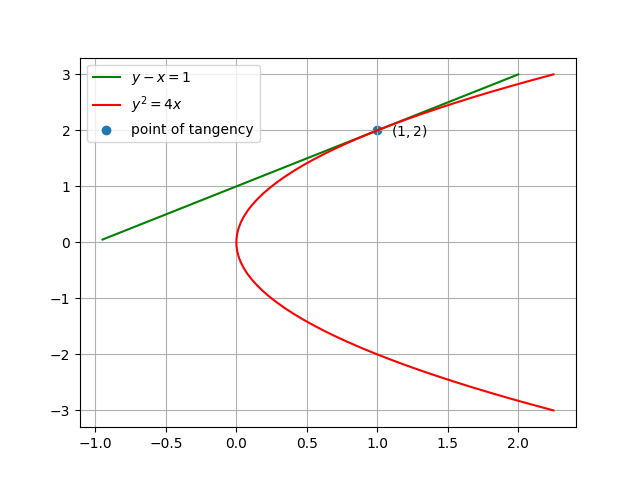
\includegraphics[width=\columnwidth]{./solutions/1/20/Figure_1.png}
	\caption{Figure depicting the point at which the line is tangent to the parabola}
	\label{eq:solutions/1/20/fig1}
\end{figure}
